%
%  This document contains chapter 2 of the thesis.
%

\renewcommand{\chptindicator}{ch2}

\setcounter{chapter}{1}
\chapter{ANALYSIS}\label{ch:analysis}
%%%%%%%% This line gets rid of page number on first page of text
\thispagestyle{empty}
%%%%%%%%%%%%%
From determining the best breakfast cereal~\cite{Curtis2021} to electing the next
president, voting is an extremely important aspect of modern society.
Nevertheless, disease, injury, and other impediments can create difficulties for
individuals participating in such democratic processes, preventing them from
expressing their voice and participating in deliberation, as well as decreasing
the overall quality of the result.
Proxy voting is a method by which participants are able to have others vote on their
behalf.
We examine the ability of proxy voting to decrease the impact of such frustrations.
We additionally determine strategies by which proxies and their constituents can
cooperate in order to reduce the change their absence would otherwise cause.
These strategies include allowing proxies and constituents to aggregate their
preference into one result, as well as determining how best to aggregate all votes
in a unified-vote/single-winner/single-dimension continuous space model.

\section{Previous Work}\label{sec:\chptindicator-previous-work}
Proxy voting is a well-discussed topic, and we build off many author's previous work.

Jonas Degrave~\cite{Degrave2014} implemented a simple model to calculate how much
weight a proxy has.
The model even allows for agents to delegate multiple proxies.
He treated proxy delegations as a digraph where nodes are voters and edges represent
delegating proxies, and created two methods to determine the weights of each proxy.
The first method constructs a linear equation for each agent, consisting of the
agent's original weight plus the weight of the agents that delegate to it.
The second employs an adjacency matrix and uses linear algebra to calculate the
solution.
Ultimately, both methods simply sum the total weight allocated to a proxy.
We will employ the first technique, since it allows for a straightforward way to
delegate voting power that would not be confusing to voters.
However, we will not take full advantage of it by disallowing proxies to delegate to
other proxies, as well as only allowing each agent to delegate one proxy.
Such proxy-to-proxy delegation is known as \textit{liquid democracy}, which has its own
challenges and advantages.
Unfortunately, it can have the effect that delegates might not know who wields their
voting power, and so we will focus on enhancing deliberation in
unified-vote/single-winner/single-dimension continuous space scenarios.

Related to weight, Zhang~and~Grossi~\cite{Zhang2022} explore treating weight as a
probability instead of a count, in addition to simply transferring voting power to
the proxy.
In the probability model, inactive agents spread their weight out amongst several
proxies.
This probability represents the odds the agent would delegate their full weight to that
proxy.
The probability model allows Zhang~and~Grossi to probabilistically predict the
outcome of a vote, and use that model to see if agents can correctly identify some
world state.
They assume that any agent is able to delegate to any other agent.
We share this assumption, though we will only focus on transferring voting power
directly instead of treating it as a probability.

Anurita~Mathur~and~Arnab~Bhattacharyya~\cite{Mathur2017} looked at several voting
mechanisms applied on a single-winner election vote and determined a ranking for
these mechanisms.
\textit{Voting mechanisms}, also known as \textit{aggregation mechanisms}, are
algorithms that take the preferences of all active voters and turn them in to the
output of the system.
They apply these mechanisms on a dataset while looking only at datapoints without a
Condorcet winner.
In their work, they say a mechanism `beats' another if it has a larger fraction of
the population prefer its output over the other's output.
They discover that the GT\footnote{
    Presumably meaning `Game Theory.'
}~method~\cite{Rivest2010} beats all others, the Schulze~method~\cite{Schulze2011}
and Minimax voting mechanisms always agree and beat all other mechanisms besides the
GT method, while Borda beats Copeland and Plurality, and Plurality comes in last.
These mechanisms are briefly described in~\autoref{tab:\chptindicator-mathur-voting-mechanisms}.
This study will also look at voting mechanisms and attempt to determine which
mechanism is best suited for proxy voting.
Our work will differ significantly from theirs, however, as we will explore voting
mechanisms used in a continuous voting space instead of a discrete-space.
Additionally, our mechanisms will be different from the ones they employed since
their mechanisms either do not work in a continuous preference space, or do not work
well with proxy voting.

\begin{table}[htbp]
    % increase table row spacing, adjust to taste
    \renewcommand{\arraystretch}{1.3}

    \caption{
        Definitions for the voting mechanisms used by~\cite{Mathur2017}.
        $n$ represents the number of candidates for some vote.
    }
    \label{tab:\chptindicator-mathur-voting-mechanisms}

    \centering
    \begin{tabular}{| r | p{0.80\linewidth} |}
    \hline
    \thead[r]{Voting \\ Mechanism} & \thead[l]{Description}  \\
    \hhline{|=|=|}
    Borda & {
        Agents rank each candidate, 1 to $n$.
        The candidate ranked first receives $n - 1$ points, the candidate in second
        $n - 2$, etc.
        Whichever candidate receives the most points total wins.
    } \\
    \hline
    Copeland & {
        Agents rank candidates 1 up to $n$.
        Agents are able to leave some blank, all of which will be counted as last place.
        After all agents have ranked the candidates, they are compared pairwise.
        If a candidate is more often ranked better than another, it gets one point.
        If they are more often ranked worse, they get 0 points.
        When the number of ranked better vs ranked worse is equal, the candidate
        receives half a point.
        The candidate with the largest score wins.
    } \\
    \hline
    GT & {
        Agents rank each candidate, and a pairwise margin matrix is generated.
        In the matrix, position $(x, y)$ is the number of rankings that prefer $x$ over
        $y$, minus the number of rankings that prefer $y$ over $x$.
        A zero-sum game is defined, and an optimal mixed strategy computed.
        % \vicki{explain the zero sum}
        A zero-sum game is a situation in which for every point gained by one side,
        the other side looses and equal number of points.
        The winner is then chosen randomly using the optimal mixed strategy.
        See~\cite{Rivest2010} for more details.
    } \\
    \hline
    Minimax & {
        Agents rank every candidate from 1 to $n$.
        Candidates are compared pairwise, where candidate $x$ is compared to
        candidate $y$.
        The score of each comparison is the number of votes candidate $y$ receives
        more than candidate $x$.
        Then, the maximum score for each candidate $x$ (meaning, its largest
        pairwise defeat) is determined.
        The candidate with the lowest (or minimum) maximum score is selected as the 
        winner.
    } \\
    \hline
    Plurality & {
        Each agent selects their favorite candidate.
        The candidate with the most votes wins.
    } \\
    \hline
    Schulze & {
        Agents rank candidates, and are allowed to skip rankings, give the same rank
        twice, or not rank a candidate.
        Candidates with the same ranking are said to be equally preferred, and
        unranked candidates are ranked last.
        Then, a weighted directed graph connecting agents is generated.
        An edge going from candidate $A$ to candidate $B$ with a weight of 10 means
        10 more agents prefer $A$ over $B$ than $B$ over $A$.
        Using this graph, multiple paths are generated between candidates.
        The strength of the path is the sum of the weight of each edge in the path,
        and the path with the highest strength from $A$ is compared to the strongest
        path from $B$.
        The same occurs with paths from $A$ to $C$, $B$ to $C$, etc.
        The candidate that has stronger paths to each individual agent than all other
        agents wins.
    } \\
    \hline
\end{tabular}

\end{table}


\etal{Cohensius}~\cite{Cohensius2017} explore the use of proxy voting in a
continuous metric space using two voting mechanisms: mean, median.
They also explore proxy voting in a binary space using majority.
They discovered proxy voting using any of these mechanisms generally produces lower
error than direct voting with active voters alone.
This is not too surprising: reintroducing information lost through inactive voters,
regardless of the method, ought to help the system.
Nevertheless, they were able to show that proxy voting is effective under a number of
symmetrical and asymmetrical preference distributions, while under both random and
strategic participation.
However, the majority of their research focuses on voting with infinite populations.
While this work would certainly be applicable to larger populations, since a
population of sufficient size will begin to behave like an infinite
population\footnote{
    Naturally, $\lim_{x \rightarrow \infty} x = \infty$.
}, we are more interested in more realistic proxy voting in smaller, finite populations.
As such, we will explore the effects of proxy voting on a finite population of this
size, as well as explore other possible voting mechanisms, inside this continuous
metric space.

\etal{Bulteau}~\cite{Bulteau2021}, develop and experiment with a framework for
aggregating preferences in several spaces using $L_p$ mechanisms.
$L_p$ aggregation methods work by minimizing the sum of distances to the power of $p$
($d^{\,p}$, where $d$ is a distance) between a possible solution and the voters'
preferences.
These mechanisms are particularly useful because they allow fine-tuning of the
aggregation method by changing $p$.
Specifically, in single-dimension single-winner continuous models, they employ $L_1$
(median),
$L_2$ (mean), and $L_{\infty}$ (mid-range, meaning the point between the highest and
lowest agent preference).
They additionally treat any possible value in the space as a potential output as the
system.
They provide a number of remarks and observations for each of these mechanisms, which
we will be borrowing.
However, they examine these mechanisms without weighted votes, which we will have.
As such, we will adapt each of the mechanisms to use weighted votes so they can work
with proxies, and examine how they operate in the continuous space.

James Miller~\cite{Miller1969} imagined a governmental system utilizing proxy voting
in 1969 as a more direct form of a representative democracy.\footnote{
    That is to say, Miller envisioned a system where individuals could directly vote
    for an issue, or elect a proxy to vote for them.
    Naturally, any democracy that uses proxy voting is a representative democracy,
    since the proxy is representing the delegator.
    Nevertheless, it can be argued that Miller's proposal could provide a more direct
    democracy since a voter can directly vote for an issue if they so choose.
}
His work focuses on reworking the current House and Senate systems entirely by using a
more directly involved populace, but his ideas can still be relevant under the current
system.
In particular, he introduces the idea we call \textit{expert proxies},
those being individuals who would `vote as [the delegator] would if only
[the delegator] had the time and knowledge to participate directly'~\cite{Miller1969}.
Additionally, Miller states `a representative should be an expert, or at least
competent, in each field [on which they are voting]'~\cite{Miller1969}.
This is true both in the government as well as other situations where decisions are
made by voting.
As such, we consider scenarios where a proxy is dubbed, at least according to its
constituents, an `expert,' and so the constituents will go with its preference
instead of their own.

\section{Preliminary Setup}\label{sec:\chptindicator-preliminary-setup}

\subsection{The Model}\label{subsec:\chptindicator-the-model}
An important part of any study is the model it uses to represent the system being
studied.
We employ a model described by \etal{Cohensius} in their 2017
article~\cite{Cohensius2017}.
This model places voters' preferences in a single-dimension continuous
metric~space~\systemspace, such as in~\autoref{fig:\chptindicator-system-metric-space}.
In this model, two points that are close together in the metric space represent
similar preferences, while two points that are far apart represent very different
preferences.
As a point moves further away from the agent's preference, the agent likes it less.
This model works best when an upper and lower bound is provided, such as only
allowing agents to vote in the interval $[-1, 1]$, to prevent agents from voting
extremely far in either direction and so potentially biasing the vote.
Not all ways of voting a susceptible to such attacks, but it regardless must be a
consideration for those that are.

The difference between multiple equidistant points in the model may not be equivalent
to the agents.
For example, an agent who must spend \$30 may prefer spending more money rather than
less.
As such, even though \$29 and \$31 are equidistant to \$30, an agent may vastly
prefer \$31 over \$29.
However, for our model, we will assume agents only care about the distance from their
preference, rather than if it is greater or less than some amount.

\begin{figure}[htbp]
    \centering
    % Built using:
% https://tex.stackexchange.com/a/148253/277236
% https://tex.stackexchange.com/a/380491/277236
\begin{tikzpicture}[scale=7.0]
    \draw(-1,0) -- (1,0) ; % Axis
    \foreach \x in {-1, 0, 1} % Numbers and lower lines
    \draw[shift={(\x,0)},color=black] (0pt,2pt) -- (0pt,0pt);
    \foreach \x in {-1, 0, 1} % Numbers and lower lines
    \draw[shift={(\x,0)},color=black] (0pt,0pt) -- (0pt,-2pt) node[below]{$\x$};

    % Labeled points
    \tkzDefPoint((-4/7), 0){agentA}
    \tkzDefPoint((3/4) , 0){agentB}
    \tkzDefPoint((1/12), 0){agentC}
    \tkzLabelPoint[above](agentA){$\truthof{a}$}
    \tkzLabelPoint[above](agentB){$\truthof{b}$}
    \tkzLabelPoint[above](agentC){$\truthof{c}$}

    \foreach \n in {agentA, agentB, agentC}
    \node at (\n)[circle,fill,inner sep=1.75pt]{};
\end{tikzpicture}
    \caption{
        Example of a 1D continuous preference metric space, where \truthof{x} represents
        the preference of agent $x$.
        The x-axis represents some preference space.
        An agent can have a preference anywhere within this space.
        One way to interpret the model is to have the leftmost point be the most
        against some idea and the rightmost point is the most in favor of the same idea.
        Importantly, points towards the center of the space are the most ambivalent,
        neutral, or central on the idea.
        Alternatively, points towards the center may also prefer some type of
        compromise or alternative solution instead.
    }
    \label{fig:\chptindicator-system-metric-space}
\end{figure}

Such a model is extremely flexible and can be interpreted in different ways.
When applied to binary for-or-against voting problems, options can be placed at either
extreme of the interval.
As an example, say shareholders at some company are voting on new data collection
policies.
As an example, say a group is choosing whether to put pineapple on pizza.
Using the interval $[-1, 1]$, we can place `no collection at all' at -1, and `heavy
collection' at 1.
Agents vote according to their preference: -1 for no collection, 1 for heavy collection.
So far, everything works the same as a normal vote.
However, due to the continuous nature of the voting space, the agents can vote
anywhere in the given interval.
Therefore, agents who don't care one way or the other can vote at 0 instead of being
forced to choose an option.
Additionally, those that are only slightly in favor (meaning they would prefer
collection but don't really care that much) can choose some value between 0 and 1.
Once the votes are aggregated, the result can be rounded to whichever option is
closest.
The continuous space allows agents to better express themselves according to what
their actual preference is, instead of being forcibly binned into one value or the
other.

Alternatively, if the majority of the options are about the center, it may be a sign
neither option is satisfactory.
Using the data collection example, we can reinterpret 0 to mean the agents don't
mind collecting users' data, but don't personally care either way.
These agents would vote around 0 to avoid imposing.
By making the agents aware of how 0 will be interpreted, they can express their
dissatisfaction by voting at or around 0.
Normally, voting goes through a bargaining and an enforcement
phase~\cite{Fearon1998}, but if a sufficient number of agents vote close to 0, the
group can reopen discussion about the topic and re-bargain before conducting a new vote.
This enhances the cooperation aspect of voting, and creates a fundamental change:
voting is no longer the end of the process, but rather part of it.

Finally, the continuous space model allows for another, very powerful interpretation:
interpreting the votes and result as continuous values.
For example, imagine Congress is voting on how much to allocate to the defense budget.
In this scenario, Congress can decide to allocate anywhere between \$0 and \$1,000.\footnote{
    Naturally, these values are not realistic and are meant to be representative.
}
A voter can place their vote anywhere between those values, and the result of the
vote can be how much Congress allocates.
Say there are three voters, each with their own preferences, and all voters are
active (no voter delegates their vote).
Agent $a$ prefers \$750, $b$ prefers \$600, and $c$ prefers \$250.
One way we could aggregate these preferences is by finding their mean.
By averaging these preferences, the system would output
$\frac{\$(750 + 600 + 250)}{3 \text{ voters}} = \frac{\$1600}{3 \text{ voters}} =
\$533.33$,
which would be the amount allocated to the defence budget.
Being able to vote on continuous problems and yield a continuous output, as well as
working with binary issues, makes the model extremely flexible and allows it to
tackle any number of problems.

We are also able to easily calculate error using a continuous space.
The error can simply be the distance from the result of the system when all agents
are active, and the result under proxy voting.

The flexibility of the continuous model in both the discrete and continuous realms, its
ability to use different voting rules, easy interpretability, and easy error
calculation are the reasons it is employed in this study.
We will focus primarily on the continuous instead of the discrete output of the
model, since observing the continuous output allows for more granularity in the
differences between proxy and non-proxy voting, as well as in the differences between
voting rules.

\subsection{Voting mechanisms}\label{subsec:\chptindicator-voting-mechanisms}
This study also makes use of \textit{voting mechanisms} or \textit{voting rules},
which are functions that map a set of preferences in~\systemspace\ to an outcome that
also exists in~\systemspace.
For these, we take inspiration from \etal{Bulteau}'s~\cite{Bulteau2021} work in
aggregating one-dimensional single-winner elections by using their $L_p$ aggregation
methods, as well as mixing in plurality.
$L_p$ aggregation methods work by minimizing the sum of distances to the power of $p$
($d^{\,p}$, where $d$ is a distance) between a possible solution and the voters'
preferences.
Naturally, since~\cite{Bulteau2021} did not use weighted proxies, these methods need
to be adjusted to allow for weight.
Below, \agentweight\ represents the weight of an agent \agent, and \systemproxies\ is
the ordered set of active voters.
Additionally, \agenttruth\ is the preference of an agent.
With these notations, the mechanisms we use are
\begin{enumerate}
    \item {
        \textit{Median ($L_1$)}, defined as
        $\textbf{md}(\systemproxies) =
    \truthof{
    \min\left\{
        \agent_i \in \systemproxies \text{ s.t. }
            \weightof{\agent_i} +
            \sum_{\agent_j \in \systemproxies}^{\agent_{i - 1}} \weightof{\agent_j}
        \geq \frac{\systemweight}{2}
    }
\right\}$.
        Essentially, the median is the active agent whose additional weight makes the
        sum of weights become equal to or greater than half the total weight of the
        system.
        The sum will occur in the same order as the ordering of voters in
        \systemproxies.
        There is an edge case when two agents share a border with half the total weight.
        In this case, the average between the preferences of the two agents is taken.
    }
    \item {
        \textit{Mean ($L_2$)}, defined as
        $\mathbf{mn}(\systemproxies) =
    \frac{1}{\systemweight}
    \sum_{\agent_i \in \systemproxies} {\weightof{\agent_i} \cdot \agent_i}$.
        This is a typical weighted average.
    }
    \item {
        \textit{Mid-range ($L_\infty$)}, defined as
        $\mathbf{mr}(\systemproxies) =
    \frac{
        \truthof{{\systemproxies}_1} + \truthof{{\systemproxies}_n}
    }
    {2}
$, meaning the preference
        of the active agent with the lowest preference plus the preference of the
        active agent with the highest preference, divided by two.
    }
\end{enumerate}
Additionally, we will apply these mechanisms against all active voters (to simulate
if proxy voting was not allowed) and all voters, both active and inactive, (to simulate
the best case where all agents vote), without any weights.
These additional calculations serve as baselines to determine how well proxy voting
works in these scenarios.

\subsection{Coordination Mechanisms}
\label{subsec:\chptindicator-coordination-mechanisms}
There are also several ways an individual proxy can agree to cast its vote own behalf
of its constituents.
Each has different advantages and disadvantages for the proxy, its constituents, and
the system as a whole.
We will examine five different `coordination' mechanisms that `groups' (meaning a
proxy and its constituents) can use:
\begin{enumerate}
    \item {
        \textit{No preference change - Expert}.
        The group applies its total weight to the proxy's preference.
    }
    \item {
        \textit{No preference change - Active Only}.
        Only active agents vote with no additional weight.
    }
    \item {
        \textit{No preference change - Cooperative Mean}.
        The group allocates its weight to the mean of the proxy's and its
        constituents' preferences.
    }
    \item {
        \textit{No preference change - Cooperative Median}.
        The group allocates its weight to the median of the proxy's and its
        constituents' preferences.
    }
    \item {
        \textit{Preference change - Expert}.
        The group applies its total weight to the proxy's preference.
        This is useful for cases when a proxy is deemed by its constituents as an
        `expert', as discussed by James Miller~\cite{Miller1969}.
        However, the proxy's preference has changed as it has participated in
        deliberation and discussion with the other active voters.
    }
    \item {
        \textit{Preference change - Expert with Consequences}.
        The proxy is an expert and the group allocates its weight to the proxy's
        preference, but the proxy's preference has changed.
        However, due to this change the proxy is only allowed to apply its own
        weight, leaving its constituents unrepresented.
        This represents situations where a proxy is considered an expert, but the
        constituents impose a condition that the proxy can only represent them if
        they vote a certain way.

        Note this is analogous to only having the active agents vote.
    }
    \item {
        \textit{Preference change - Cooperative Mean}.
        The group allocates its weight to the mean of the proxy's and its
        constituents' preferences.
        However, the proxy's preference has changed as it has participated in
        deliberation and discussion with the other active voters.
    }
    \item {
        \textit{Preference change - Cooperative Median}.
        The group allocates its weight to the median of the proxy's and its
        constituents' preferences.
        However, preferences have changed due to deliberation.
    }
\end{enumerate}
These mechanisms are used in an attempt to simulate real-world consequences of proxy
voting, as well as identify potential techniques to deter or mitigate a proxy's
ability to swing the system by aggregating a large amount of weight and abusing it.

\section{Assumptions}\label{sec:assumptions}
In order to conduct this study, we make a number of assumptions.
First, we assume that voting issues are one off, meaning agents vote on only one
topic at a time.
This allows agents to select a proxy that works best for the current topic instead of
selecting the best proxy for all topics.

Additionally, we only consider scenarios where unified-vote proxy voting is used, where
the proxy receives the voting power of the delegating voter, increasing their weight,
and proceeds to allocate all their weight towards one vote instead of relaying their
constituents' vote.
This type of proxy voting also allows the proxy to update their (and by extension, their
constituents') preferences as new information becomes available.
While unified-vote proxy voting gives substantial flexibility to the proxy to operate
on behalf of their constituents, this flexibility requires the delegating voter to
choose a proxy who they trust to vote as close to how they themselves would.
This is a process similar to selecting experts, as described by~\cite{Miller1969}
and~\cite{Mueller1972}.
By using unified-vote proxy voting instead of relay-style voting, we hope to exploit
the advantages of proxy voting that the relay-style does not provide.

We also assume that each voter has reasonable knowledge of potential proxies'
opinions, meaning they have a decent idea of the preferences of other proxies.
This will allow them to choose the proxy that has the opinion most similar to their own.
While in reality voters will likely not have perfect knowledge of others' opinions,
it is often not particularly difficult to gauge the opinion of others, especially
those with whom an individual often associates, and so we believe this assumption is
reasonable.

Finally, we assume that there are no factors besides closeness in opinion that affect
the choice of proxy.
This differs from some systems, such as that presently used by the House of
Representatives which includes restrictions such as a proxy can only serve ten
voters~\cite{CERP2020}.
However, we feel removing restrictions such as these leads to a more interesting
discussion, since it allows the use of different voting mechanisms and more extreme
cases.

\section{Contribution}\label{sec:\chptindicator-contribution}
We explore proxy voting in a unified-vote/single-winner single-dimension
continuous space model.
We employ three well-known $L_p$ mechanisms, specifically
\begin{enumerate}
    \item {
        Median ($L_1$)
    }
    \item {
        Mean ($L_2$)
    }
    \item {
        Mid-range ($L_\infty$)
    }
\end{enumerate}
Each of these mechanisms will additionally be applied to direct voting with all
agents and direct voting with only those agents that are present.
This is done to show what the output of the system would be with all information
(direct voting with all agents), as well as the output with minimum information
(direct voting with only those agents that are present).
The error will be the distance between the result and direct voting with all agents.

We will additionally apply what we've dubbed `coordination mechanisms,' which are
techniques by which proxies and constituents work together to determine how their
weight will be allocated, meaning how the proxy will vote on their behalf.
The mechanisms we will explore are described
in~\autoref{subsec:\chptindicator-coordination-mechanisms}.
These mechanisms are used in an attempt to simulate real-world consequences of proxy
voting, as well as identify potential techniques to deter or mitigate a proxy's
ability to swing the system by aggregating a large amount of weight and abusing it.

Whereas voting on a continuous interval is uncommon and finding a real world dataset
using preferences on an interval currently does not seem possible, these investigations
are performed using preferences generated from several statistical distributions.
We will use various distributions to allow the gathered data to represent
different distributions of voters in the real world.
These distributions include well-known statistical distributions, such as the uniform
distribution, the Gaussian distribution, as well as a few beta distributions.
The distributions used and their notations are listed
in~\autoref{tab:\chptindicator-distributions-used}.
% \vicki{Why is normal indifferent?  Define the beta distribution.}
% MDH: The normal distribution can be characterized as indifferent or centralist
% because many of the votes are about the center. In reality, each of these
% distributions could represent any number of different population types; I'm just
% providing potential types so the reader doesn't need to on their own. I've added a
% sentence clarifying this in the table caption.
% The beta distribution is a well-known statistical distribution. I'm using it
% because it can easily create diverse shapes by tweaking its parameters. I've added
% a sentence clarifying these distributions are well-known.

\begin{table}[!htbp]
    % increase table row spacing, adjust to taste
    \renewcommand{\arraystretch}{1.3}

    \caption{
        The distributions to be used to generate preferences.
        Note how each distribution represents a population type.
        These types are representative, and any distribution could potentially
        represent a different population type that shares the same shape as the
        distribution.
        Additionally, any skewed distributions can be inverted to create a
        distribution that is skewed in the other direction (e.g. a distribution
        skewed in favor can be inverted to create a flipped distribution skewed
        against).
    }
    \label{tab:\chptindicator-distributions-used}

    \centering
    \begin{tabular}{|r|l|c|l|}
    \hline
    \thead{Distribution} & \thead{Notation} & \thead{Symmetrical?} & \thead{Population Type}
    \\
    \hhline{|=|=|=|=|}
    Uniform & \uniform{-1}{1} & \ding{51} & Evenly spread
    \\
    \hline
    Normal/Gaussian & \gaussian{0}{\sfrac{1}{3}} & \ding{51} & Mostly
    centrist/indifferent
    \\
    \hline
    Beta(0.3, 0.3) & \betadistribution{0.3}{0.3} & \ding{51} & At either extreme
    \\
    \hline
    Beta(50, 50) & \betadistribution{50}{50} & \ding{51} & Strongly
    centrist/indifferent
    \\
    \hline
    Beta(4, 1) & \betadistribution{4}{1} & \ding{55} & Skewed in favor
    \\
    \hline
\end{tabular}
\end{table}

Each experiment will have a population of 24.
We chose this number because prior experimentation shows it to be a good balance
between having few enough agents that an agent going inactive can change the
results, while not so few that there are an agent going inactive is catastrophic.
Since having no delegates or all delegates would not be interesting, we will
experiment with 1 to 23 delegating agents and examine how error correlates with
the number of delegators.

For each experiment, agents will choose some preference using the current distribution.
Afterwards, one agent will become inactive and choose the closest active agent to be
their proxy.
Following this, the proxies and their constituents will apply a coordination
mechanism, and each voting mechanism will be applied.
The next coordination mechanism will be used, then each voting mechanism will be
applied again.
Once all coordination mechanisms have been used, the number of inactive agents will
increase until all but one agent is inactive.
Finally, agents will select a new preference from the next distribution and the
process will begin again.
This will continue until all possible combinations have been used.

We will show that proxy voting with the right combination of mechanisms generally
yields considerably lower error than active-only voting.
We also show proxy voting is beneficial even when agents' preferences change.
However, proxy voting appears to be least effective on highly-polarized topics.

\section{Results}\label{sec:results}

\subsection{Mechanism Combinations}\label{subsec:mechanism-combinations}
The absolute mean error as a percent of the total preference space by coordination
mechanism per voting mechanism is graphed in
\autoref{fig:vm-col-cm-hue-error-as-percent-of-space-abs-mean}.
% 04/13: \vicki{Briefly describe how you define mean square error}
The absolute mean error as a percent of the total preference space  \vicki{Why sigma?  Sigma normally means standard deviation.  Mean squared error is typically MSE.}
$\sigma_{\lvert M\% \rvert}$  is defined as
$
    \sigma_{\lvert M\% \rvert} =
    \frac{1}{n (\systemspace_{\max} - \systemspace_{\min})}
        \sum^{n}_{i = 1}{\lvert \epsilon_i  \rvert}
$,
where $n$ is the number of runs, $\systemspace_{\max}$ and $\systemspace_{\min}$ are
the maximum and minimum value in the preference space, respectively, and $\epsilon_i$
is the error of run $i$.
Error is defined as $\truthof{\text{proxy}}~-~\truthof{\text{baseline}}$, meaning the
output of the proxy run minus the output of the baseline (all agents voting).  \vicki{T(proxy) seems a little odd because the test doesn't always use a proxy voter.  Could use say T(test)?}

From this plot, there are a few trends that are immediately identifiable.
First, error unsurprisingly increases as the number of inactive agents increases.
This is true with two notable exceptions: first, the Active Only/Median
mechanism combination has a somewhat sawtooth shape.
This is due to the Median mechanisms always choosing a specific agent's preference
instead of aggregating to some more preferential in-between value.  \vicki{I thought it was an average if a unique median couldn't be found.  Have you considered running with 25 agents, so the median is always clear?}

The second exception is that Mean coordination mechanism consistently dips when all but
one agent become delegators. 
\vicki{I thought you removed this case?  Did I misunderstand?  The charts look like you went until 23/24 were delegates.}
This is because we take the mean of the constituents and the proxy, then apply the
voting mechanism on the set of proxy-constituent votes.
Since there is only one agent, there is only one proxy-constituent vote and so the
result of the vote is the result of the coordination mechanism.
Essentially, the coordination mechanism replaces the voting mechanism.

We can also see the Mean and Median coordination mechanisms generally yield similar
amounts of error.
In particular, when either of these mechanisms is combined with the Mean voting
mechanism the results are very similar to when all agents are active and able to vote.

Notably, the Expert coordination mechanism exhibits higher error than the others as the number
of delegators reaches a significant portion of the population.
In particular, the Expert mechanism tracks nearly identically to Active Only when
using the Midrange voting mechanism.
Depending on the use case, this may or may not be beneficial.
If we are attempting to find the best result for all agents, this mechanism may yield
undesirable results.
However, if we are attempting to exploit the expert's experience, as described
by~\cite{Miller1969}, this error could actually be considered an improvement over
the original result.
This is because the experts were able to influence and change the vote, presumably
bringing it closer to what their expertise dictates.
Nevertheless, when the number of delegators is low, the Expert mechanism works
similarly to the other coordination mechanisms.

Importantly, it is clear that using proxy voting, regardless of the mechanisms used,
is better than losing information by not allowing inactive agents to vote in any way.

\subsection{Inactive Penalty}\label{subsec:inactive-penalty}
What if we were to introduce some penalty for the inactive agents?
Since they aren't participating as much, perhaps it would be fair that their voice is
not as strong.
We repeated the same experiments as above with different weights between a proxy and
their constituents.
Specifically, the proxies maintain their weight of 1, while their constituents have
their weight reduced to $\sfrac{1}{5}$ (0.2) of their original weight.
We choose $\sfrac{1}{5}$ because it still allows constituents to have some impact
while still having their influence significantly reduced.
The difference between all agents voting and proxy voting of such a setup are
shown in~\autoref{fig:different-weight-comparison}.
% 04/13:
% \vicki{
%     How do you define error in this case?
%     If you only give them a .2 vote, but compare to when they get a full vote, that
%     seems meaningless.
%     We are giving them a .2 vote because their vote shouldn't count as much.
%     Can you compare the shift in results between the two methods?
%     I wouldn't call it an error, but the difference between the methods.
%     Better to have the comparison between the two on one graph rather than
%     having the reader compare two figures.
% }

\begin{landscape}
    \begin{figure}[p]
        \centering
        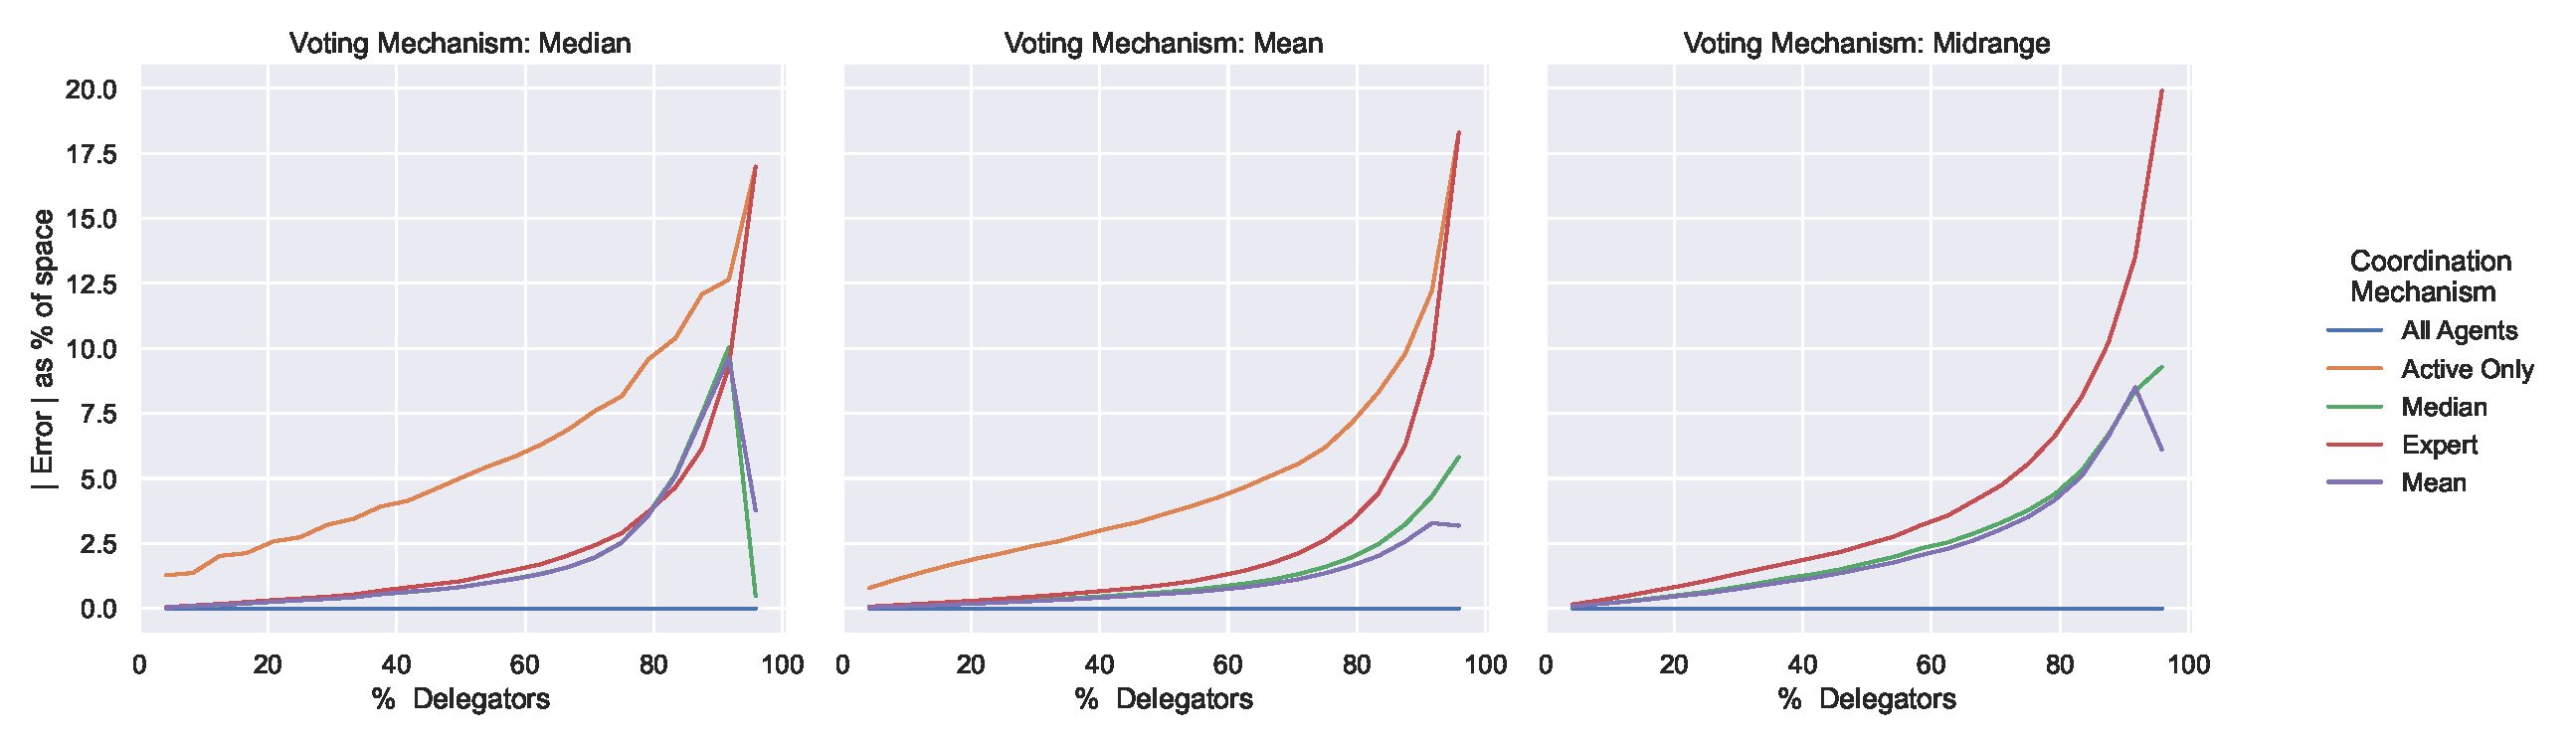
\includegraphics[scale=0.55]
        {content/chapter2/figures/vm_col_cm_hue_error_as_percent_of_space_abs_mean}
        \caption{
            The absolute mean error as a percent of the preference space by
            coordination mechanism per voting mechanism.
            `Error as a percent of the preference space' means the error divided by
            the total size of the preference space.
            Note All Agents represents when all agents are voting, meaning no proxy
            voting is used and all agents are present.
            Similarly, Active Only represents when proxy voting is not used and not
            all agents are present, and when proxies lose their constituents.
            The results are averaged over 1024 total runs.
            There are 24 total agents.
        }
        \label{fig:vm-col-cm-hue-error-as-percent-of-space-abs-mean}
    \end{figure}
\end{landscape}

\autoref{fig:different-weight-comparison}~shows there is an immediate difference from
when all agents have the same weight.
This is because, due to the weight, there is a shift towards the proxies' preferences
instead of the inactive voters'.
% 04/13: \vicki{which graphs are you referring to?  due to what?  unclear.}
% MDH: The referred-to graphs are specified in the previous sentence.
% I've re-referenced it here for clarification.
% The explanation for the error is in the next sentence.
Depending on the situation, this may be desirable.
Since the inactive agents are not participating they may not have as much information
and so their preference may not be as `up-to-date' as those who are actively
participating.
In situations where new information is constantly being introduced, such penalties
could be very valuable to ensure the most current information is being used.

Notably, the Median voting mechanism suddenly takes a sharp dip and produces a result
closer to all agents voting when using different weights than when using the same
weight.
This is strange since it is completely different compared to how any other
combination, or even the same combinations with less inactive voters, works.
With some inspection, one can find this dip is due to active voters having a
significantly larger influence compared to inactive voters.
With this setup, an active voter is worth 5 times the amount of weight than an
inactive voter.
Therefore, when an active voter's weight is added to the sum it is more able to push
the sum over the half-way mark, thereby making that active voter's preference the
median.
This is also why we see the most extreme dip with using the Median voting mechanism
with Median coordination mechanism: the proxy is able to reach the median both when
coordinating and when voting, thereby making the proxy and its constituents' vote be the
proxy's preference.
This makes the system less volatile, since votes are less likely to be an inactive
voter's, and so we don't see the large spike in error when a large percent of agents
are delegating.

Additionally, from~\autoref{fig:different-weight-comparison}, we see both the Median
and Mean voting mechanisms quickly increase
% 4/26/2023: \vicki{quickly increase in error? explain.  This is interesting as more
% delegators slows the affect. Better if x axis goes to 100\% as the other tables do.}
in difference before beginning to level out.
This is again due to the difference in weight between the active and inactive voters.
When both types of voters have the same weight, the coordination mechanisms help
ensure the loss of preference from the agent going inactive is minimal.
However, when they have different weights, in particular when the weight of the
inactive voters is substantially less than that of the actives, the results are more
akin to when the voter doesn't vote.

The Midrange voting mechanism, however, does not increase as quickly and does not
achieve as much of a difference.
Midrange, or $L_{\infty}$, takes the highest and lowest voting and averages the two.
This means it ignores weight, which is likely why the change in weights does not
affect it as much.
Any difference in the outcome, then, must come from the coordination mechanisms used
prior to the final vote being calculated with Midrange.

Notably, the Median mechanisms, both voting and coordination, yields the largest
change.
Mean is close behind, and Expert yields slightly less.
Since the Median voting mechanism has already been shown to be difficult to
manipulate~\cite{Moulin1980}, using both a Median voting and Median coordination
mechanism would likely be a good choice when choosing which mechanisms to use.

\begin{landscape}
    \begin{figure}[p]
        \centering
        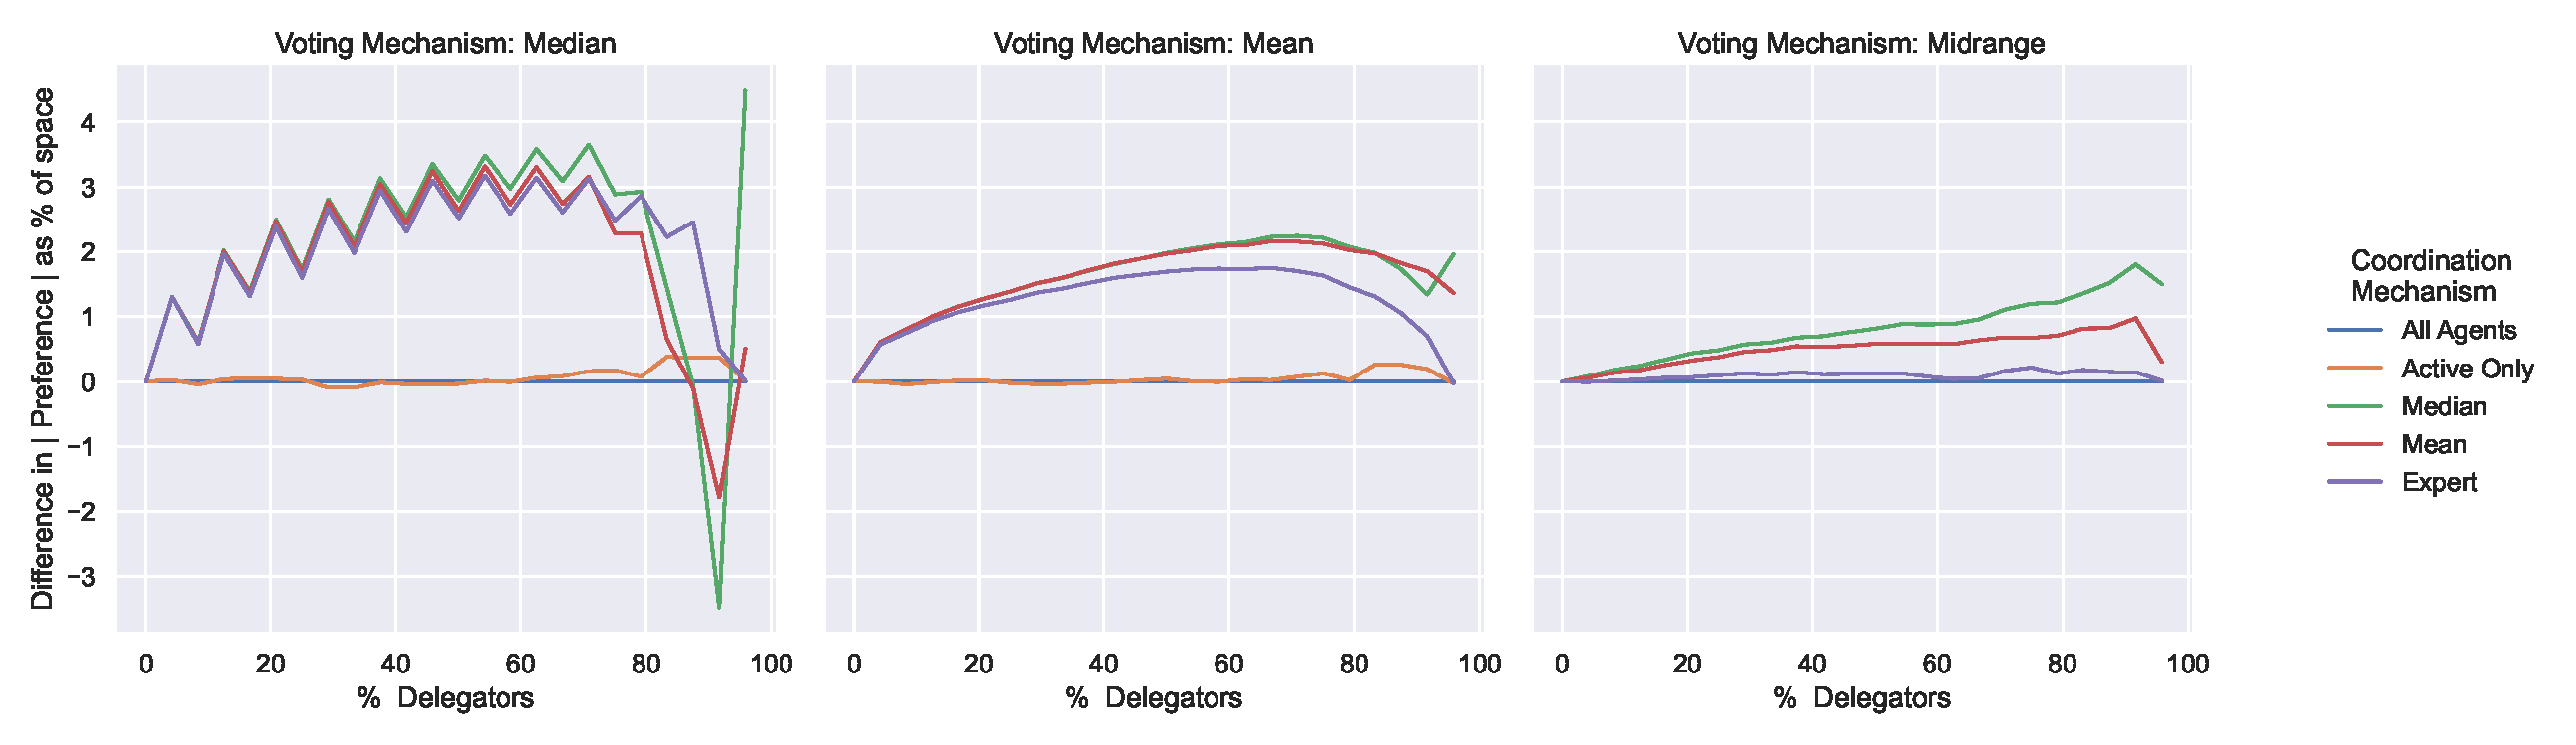
\includegraphics[scale=0.55]
        {content/chapter2/figures/different_weight/difference_abs_pref_percent_of_space}
        \caption{
            The difference between all agents having the same weight and inactive
            agents having only $\sfrac{1}{5}$ the weight as their proxies.
            The difference is in terms of distance as a percent of the preference
            space from all agents voting.
            `Distance as a percent of the preference space' means the absolute
            difference divided by the total size of the preference space.
            The results are averaged over 1024 total runs.
            There are 24 total agents.
        }
        \label{fig:different-weight-comparison}
    \end{figure}
\end{landscape}

\subsection{By Distribution}\label{subsec:results-distribution}
\autoref{fig:distribution-error-as-percent-of-space-abs-mean} shows
the absolute error as a percent of the preference space by coordination mechanism for
each voting mechanism and preference distribution.
\autoref{fig:distribution-different-scale-error-as-percent-of-space-abs-mean} shows
the same graphs, but with a different scale for each plot to more easily see the shape.
Additionally, each graph is zoomed in for readability
in~\autoref{apx:error-by-dist-zoomed}.

\vicki{Having three different versions of the same thing is painful when you are looking online, as you can't easily flip back and forth (or see them side by side). }

\begin{figure}[p]
    \centering
    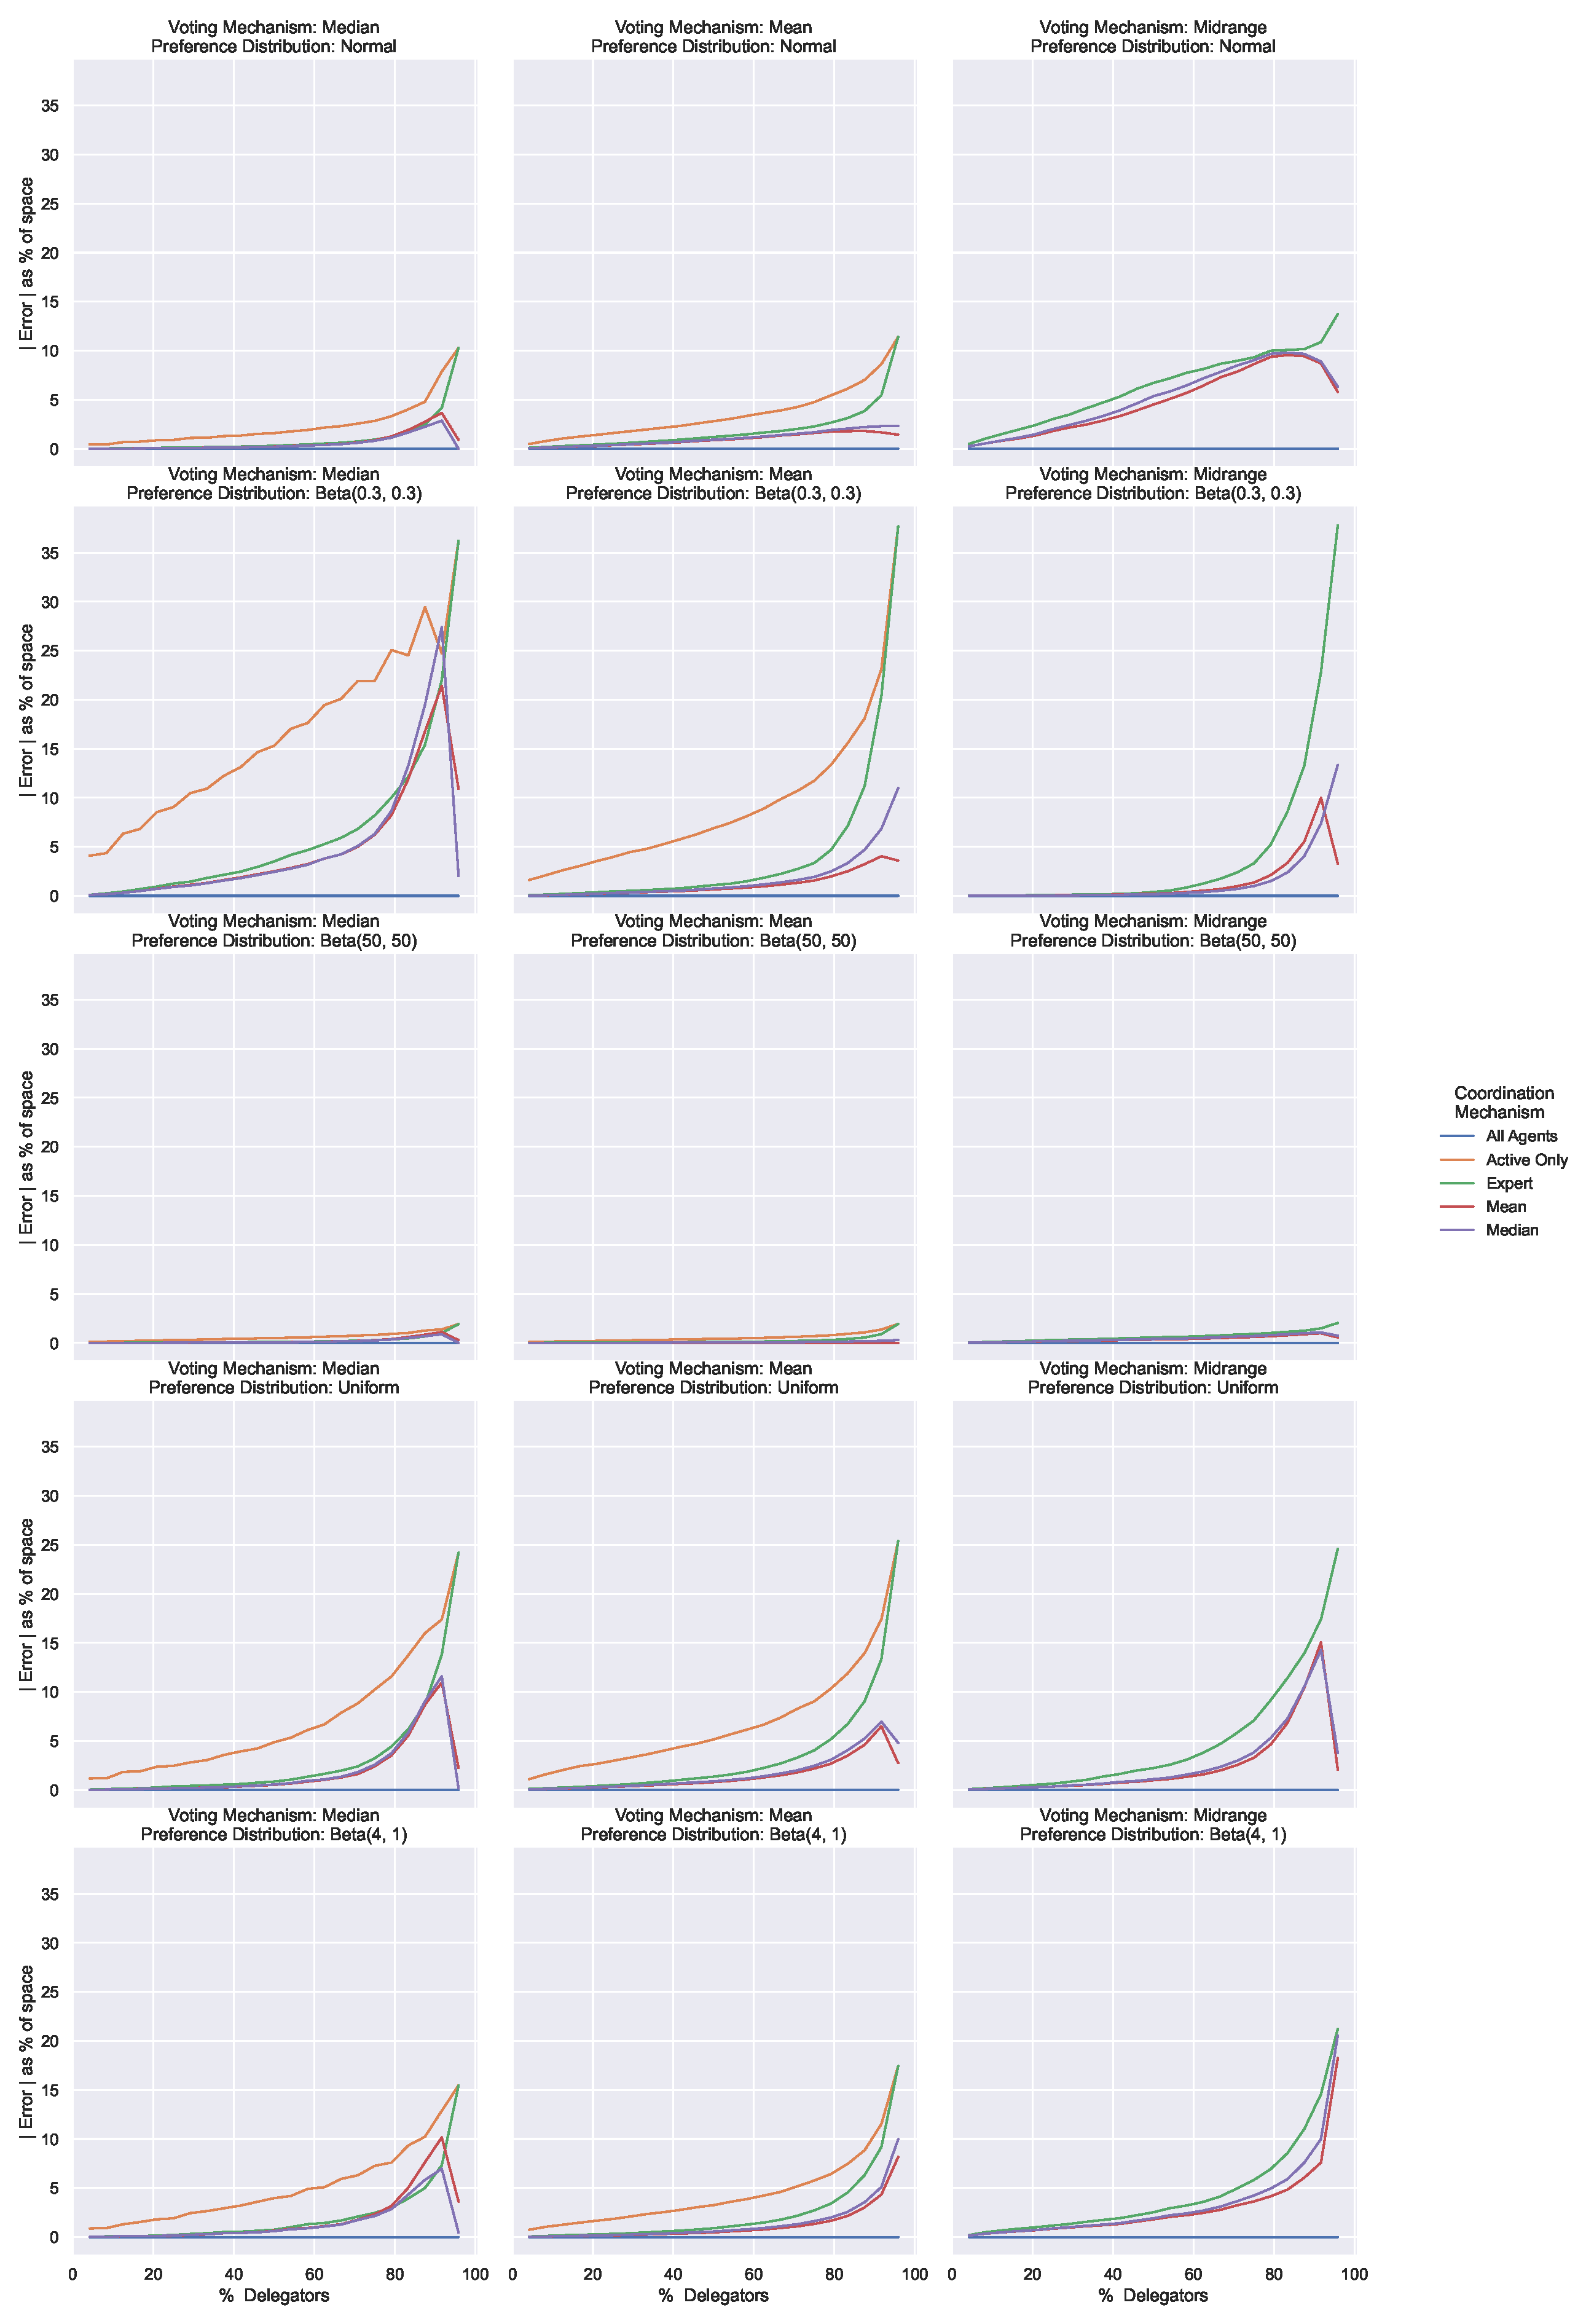
\includegraphics[scale=0.35]
    {content/chapter2/figures/distribution_error_as_percent_of_space_abs_mean}
    \caption{
        The absolute error as a percent of the preference space by coordination
        mechanism for each voting mechanism and preference distribution.
        The results are averaged over 1024 total runs.
        There are 24 total agents.
    }
    \label{fig:distribution-error-as-percent-of-space-abs-mean}
\end{figure}

Unsurprisingly, the tighter the probability density function (PDF) of a distribution,
the less error it has overall due to many votes being close to each other.
\betadistribution{50}{50} and Normal are two such distributions.
Nevertheless, these plots show the increase in error is consistent regardless of the
mechanisms or distributions used.
Mean and Median coordination mechanisms show a similar amount of error, while Expert
shows slightly more except when a large portion of the population is delegating and
when using the Midrange voting mechanism.
Interestingly, this seems to indicate again that it does not matter how you do proxy
voting so long as it is done.
Additionally, it should be noted the mechanisms perform well on most preference
distributions, including the asymmetrical distribution \betadistribution{4}{1}.

Unfortunately, while the error for other distributions is relatively similar,
\betadistribution{0.3}{0.3} yields considerably more error and starts accumulating
this error earlier when using the median voting mechanism.
\betadistribution{0.3}{0.3} represents a highly polarized topic, with its probability
density function having large spikes at either end of the preference space, making it
extremely important to ensure results are fair and accurate.
This would indicate that proxy voting, while it is still better than active-only
voting, does not work quite as well when agents have stronger, opposing opinions.

\vicki{  When you have a polarized topic, the answer chosen will always be a long distance from the preference.  For strong preferences, I'm guessing the mean or median is very volatile - changing dramatically from test to test, especially when the test size is small.  If the result changes wildly from test to test, we can hardly expect a different mechanism to change in the same wild way.  Is there a way we could verify this, say look at the standard deviation of resultant preference for the 1024 tests?   My guess is that for a normal distribution, the results are similar (for the same test, no proxy) from run to run, but that isn't true for other distributions. }

% 04/13:
% \vicki{
%     Why does this happen?
%     Is it because there are so few voters?
%     It would seem that two strong opinions shouldn't cause more error.
%     This needs to be explored as two opposing opinions is a common case.
% }
% MDH: See the following paragraphs where I explain why this could be.
% I've made a slight edit to specify this error really only occurs with the median
% voting mechanism.

For the median mechanism voting mechanism \vicki{specify the distribution}, the increase in error makes sense.
The median will most often be the preference of a specific agent, instead of some
value in between.
As such, the result will often be in one of the spikes in the PDF, since that is
where the majority of the agents' preferences will be, yielding higher error than when
using the Mean or Midrange voting mechanisms.
With the other voting mechanisms, the error is similar to other distributions using
the same mechanisms until the vast majority of the agents are inactive.
The increase in error is because as more agents go inactive there are fewer agents able
to serve as proxies, and so there may not be as desirable of a proxy to represent
each agent.

This finding is particularly important, as often the most polarizing topics are the
most important to individuals.
While it is still more beneficial to use proxy voting than not, in these polarized
cases, agents should make an extra effort to participate in-person to learn all they
can about the topic and ensure their voice is heard.
Those using proxy voting on split issues ought to be aware of this weakness and
implement some limitation to prevent inaccurate results.
These limitations could include requiring some percentage of the population, say
20--30\%, to be active.
Alternatively, if it becomes apparent that discussion is changing the opinions of the
active voters, which could be learned by occasionally polling the participants, it
may be wise to require voters to attend in person.
That way, those who have not been present to attend the deliberations can properly
participate.

\subsection{Preference Change}\label{subsec:results-shift}
\autoref{fig:abs-diff-from-preference-change-error-as-percent-of-space-abs-mean} shows
the difference in error between when proxies do have a preference change and when
they don't.
In this case, the proxies were able to shift their preferences by up to 10\% of the
total preference space, while delegators kept their original preference.
This represents the proxies changing their preference for an issue after deliberation.
\vicki{Explain how they change preference.  Are they influenced by the distribution?  I would guess if they were an outlier and changed preference, they would become more centrist.  Is this how you set it up?  If the changes are random, it doesn't seem realistic.}

Unsurprisingly, the amount of error increases as more agents become inactive.
However, the coordination mechanisms are much more tightly grouped than in other
scenarios.
We also see all voting mechanisms actually yield worse error than active-only
voting when using the Median and Mean coordination mechanisms.
This might be because delegators are selecting proxies who then shift a large amount,
leaving the delegator unsatisfied.

This potentially worse outcome highlights not only the importance of actively
participating in discussions, but also that when one needs to choose a proxy the
proxy must be someone who would act as the delegator who want them to act.

\begin{landscape}
    \begin{figure}[p]
        \centering
        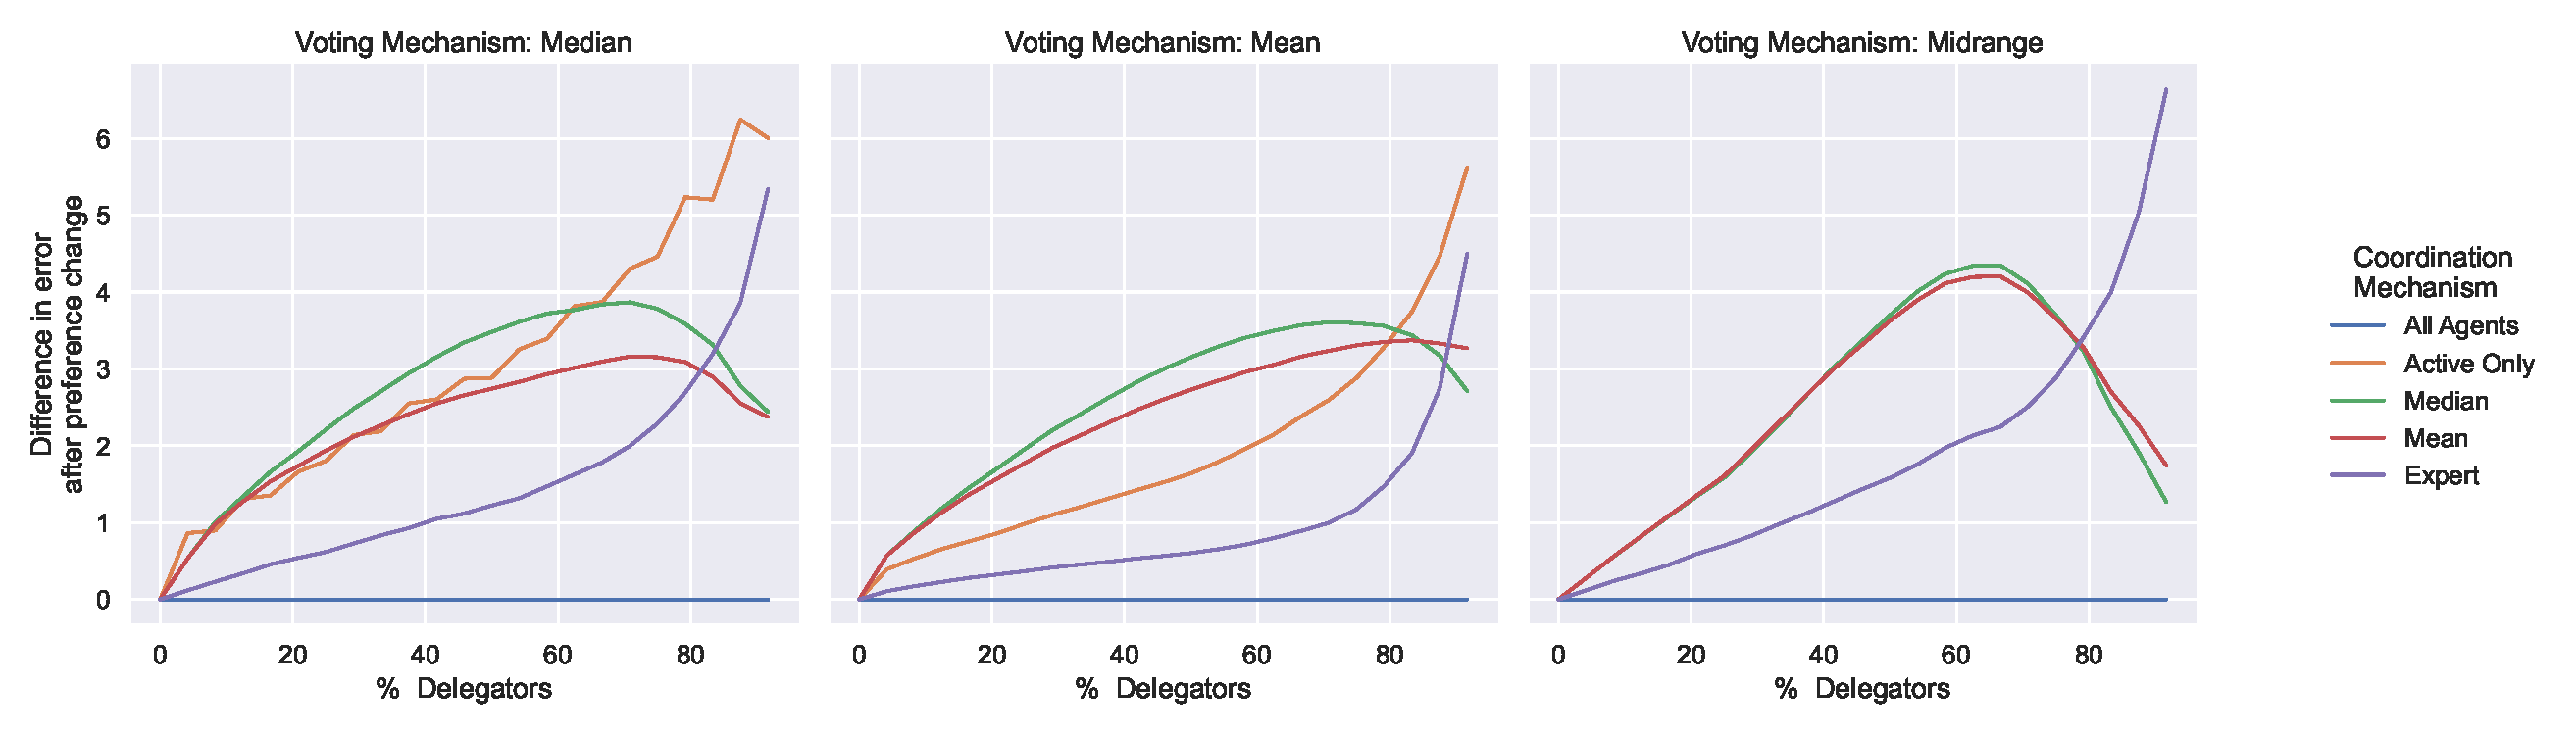
\includegraphics[scale=0.55]
        {content/chapter2/figures/abs_diff_from_preference_change_error_as_percent_of_space_abs_mean}
        \caption{
            The absolute difference in the error produced between without a
            preference change and with a preference change as a percent of space.
            The results are averaged over 1024 total runs.
            There are 24 total agents.
        }
        \label{fig:abs-diff-from-preference-change-error-as-percent-of-space-abs-mean}
    \end{figure}
\end{landscape}

\section{Conclusions}\label{sec:conclusions}
We have shown proxy voting is able to produce low-error results, even when the
delegating portion of the population is large.
We have additionally shown the Mean voting mechanism with the Mean and Median
coordination mechanisms achieve the lowest error.
These mechanism combinations are generally able to produce results with less than a 5\%
change in outcome when the delegating portion is more than half the total
population and produce considerably less when the delegating portion is lower.

We have additionally shown proxy voting is at its weakest with highly polarized
topics, such as those represented by \betadistribution{0.3}{0.3}.
In these cases, agents should make an extra effort to participate in deliberation and
vote in person instead of by proxy.

However, while proxy voting certainly makes it easier for agents to be represented,
agents should be strongly encouraged or required to participate in deliberations that
may alter their preferences.
When a proxy performs this work on behalf of an agent, the outcome of the vote may
introduce more error than would otherwise be seen with only active voters participating.

Finally, we have shown that proxy voting is a powerful tool that consistently
performs better than not allowing inactive agents to vote.
By employing proxy voting, systems will be able to maintain their accuracy while
increasing the total system utility.


% Endmatter
% For BibTeX references: specify a .bib file and a style.
% The style used here is for IEEE transactions formatting:

% Single paper format
% \references{references/IEEEabrv,references/research}{IEEEtran}

% Multi paper format
\pagebreak
\bibliographystyle{IEEEtran}
\bibliography{references/IEEEabrv,references/research}

